\renewcommand\refname{Literaturverzeichnis}
\addcontentsline{toc}{section}{Literaturverzeichnis}
\printbibliography
\cleardoublepage
\listoffigures


\clearpage

\appendix

\section{Aufgabenstellung}
\begin{figure}[h]
    \centering
    \begin{minipage}[b]{0.8\textwidth}
        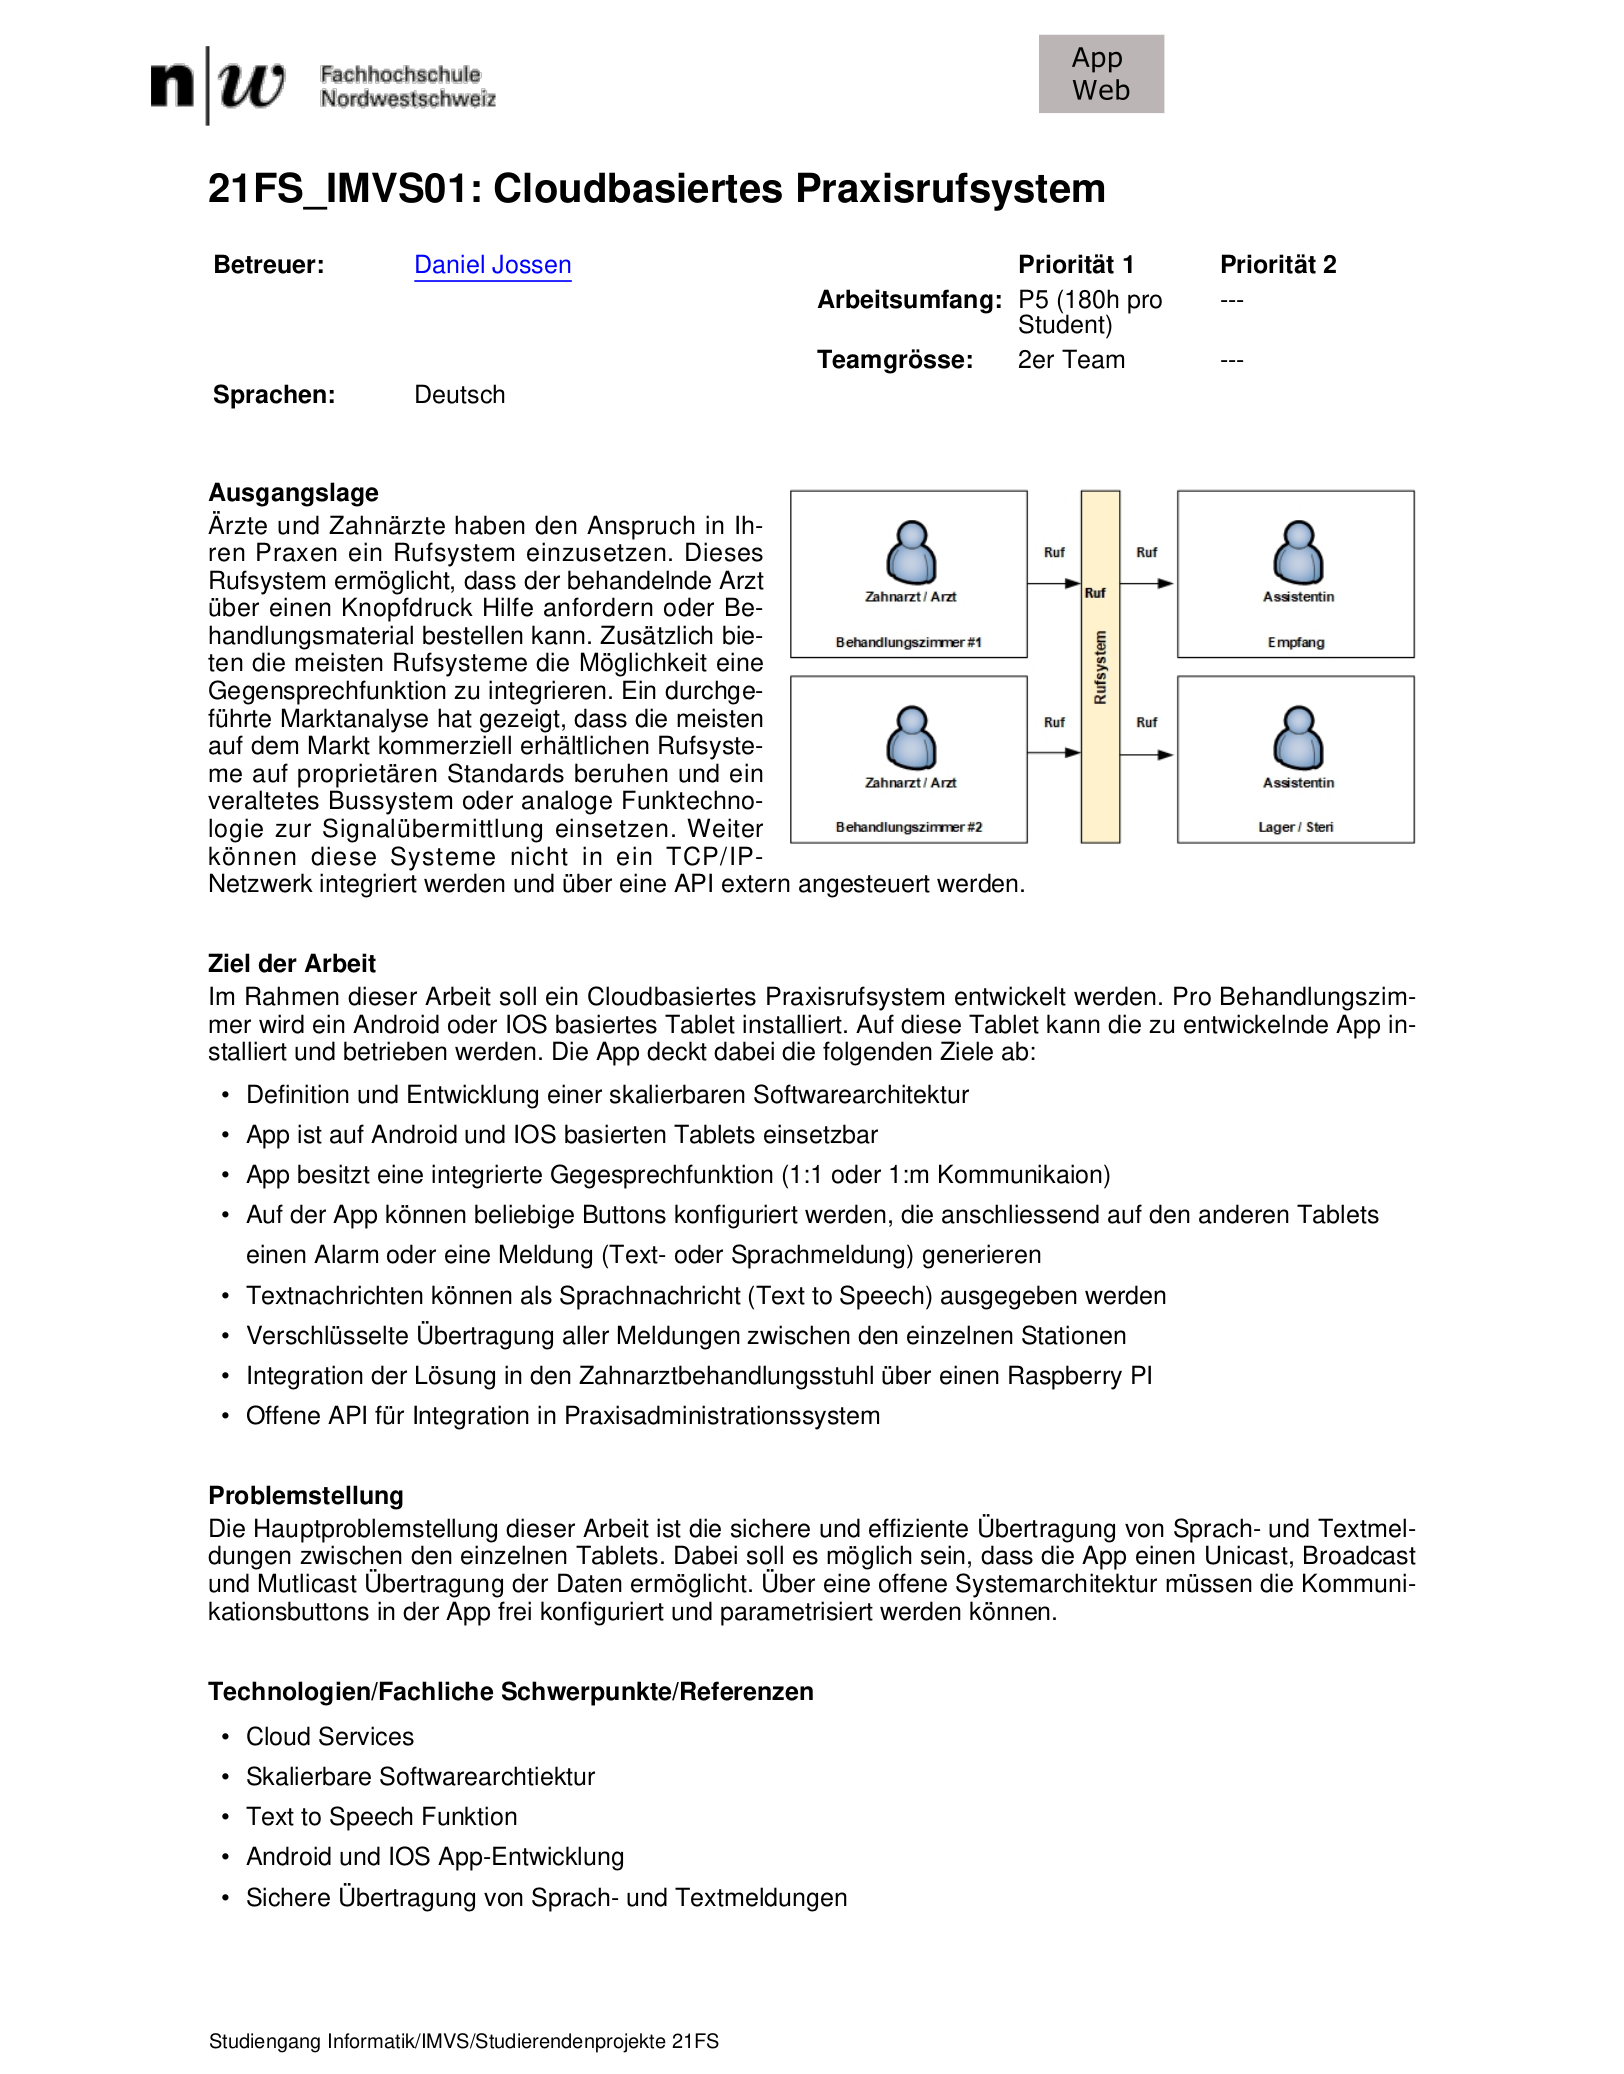
\includegraphics[width=\textwidth]{graphics/aufgabenstellung}
        \caption{Aufgabenstellung}
    \end{minipage}
\end{figure}

\clearpage


\section{Quellcodeverwaltung}

Sämtlicher Quellcode der im Rahmen des Projektes entsteht, wurde mit Git verwaltet. Der Quellcode ist für Berechtigte unter dem Projekt IP5-Cloudbasiertes-Praxisrufsystem auf github.com einsehbar.
(Referenz https://github.com/IP5-Cloudbasiertes-Praxisrufsystem). Berechtigungen können bei Joshua Villing oder Kevin Zellweger angefordert werden.


\section{Benutzerhandbuch}

\subsubsection*{Mobile Client}

\textbf{Anmeldung und Konfiguration}

\begin{enumerate}
    \item Mobile Client Applikation öffnen
    \item Anmeldedaten eingeben und bestätigen
    \item Gewünschte Konfiguration auswählen
\end{enumerate}

\textbf{Benachrichtigung empfangen}

\begin{enumerate}
    \item In Mobile Client anmelden.
    \item In Navigationsleiste (unten) "Home" auswählen.
    \item Button mit dem gewünschten Titel antippen.
    \item Die Benachrichtigung wird automatisch versendet.
\end{enumerate}

\textbf{Benachrichtigung Auflisten und Quittieren}

\begin{enumerate}
    \item In Mobile Client anmelden.
    \item In Navigationsleiste (unten) "Inbox" auswählen.
    \item In dieser Ansicht sehen Sie alle empfangenen noch nicht quittierten Benachrichtigungen.
    \item Zum Quittieren einer Benachrichtigung kann diese angetippt werden.
\end{enumerate}

\textbf{Abmeldung}

\begin{enumerate}
    \item Mobile Client Applikation öffnen
    \item Auf den Namen in der Kopfleiste tippen
    \item Logout bestätigen
\end{enumerate}

\subsubsection*{Admin UI}

\textbf{Anmeldung}

\begin{enumerate}
    \item Admin UI im Browser öffnen
    \item Anmeldedaten eingeben und bestätigen. Die Anmeldedaten erhalten Sie nach Installation des Systems vom Betreiber.
\end{enumerate}

\textbf{Einträge hinzufügen}
\begin{enumerate}
    \item Melden Sie sich im Admin UI an.
    \item Wählen Sie auf der Linken Seite die Kategorie die Sie verwalten möchten.
    \item Auf dieser Seite können Sie nun Einträge zur gewählten Kategorie verwalten:
    \begin{itemize}
        \item Klicken Sie oben rechts auf die Schaltfläche "Create" um einen neuen Eintrag zu erstellen.
        \item Klicken Sie auf einen Eintrag in der Liste um ihn zu bearbeiten.
        \item Klicken Sie die Checkbox auf der Linken Seite eines Eintrages und dann auf die Schaltfläche "löschen" um einen Eintrag zu löschen.
    \end{itemize}
\end{enumerate}

\textbf{Praxisruf konfigurieren}
\begin{enumerate}
    \item Melden Sie sich im Admin UI an.
    \item Erfassen Sie in der Kategorie "User" pro Praxiszimmer einen Benutzer.
    \item Erfassen Sie in der Kategorie "Client" pro Gerät und Zimmer einen Eintrag und weisen Sie ihn dem Benutzer des entsprechenden Zimmers zu.
    \item Erfassen Sie in der Kategorie "Notification Types" alle Benachrichtigungen die Sie zur Verfügung stellen möchten.
    \item Erfassen Sie in der Kategorie "Configurations" pro Gerät und Zimmer einen Eintrag und weisen es dem entsprechenden Client zu.
    \item Unter Notification Types können die Benachrichtigungen auswählen, die auf diesem Gerät zum Versenden verfügbar sind.
    \item Unter Rule Parameters können Sie Regeln definieren, welche Benachrichtigungen diesem Client zugestellt werden.
\end{enumerate}


\section{Installationsanleitung}

\subsubsection*{Mobile Client}
\textbf{TODO}
?? Cloud Service url configuration \\
?? FCM Integration configuration \\

\subsubsection*{Admin UI}
\begin{enumerate}
    \item Setup Amplify
    \item Setup Domain
\end{enumerate}

\subsubsection*{Cloud Service}

\begin{enumerate}
    \item Setup FCM
    \item Setup Beanstalk
    \item Pipeline
    \item Setupt RDS
    \item Setup Domain
    \item Setup EB
    \item Configure Environment
    \item Create administrator
\end{enumerate}

\clearpage
\section{Ehrlichkeitserklärung}

«Hiermit erkläre ich, die vorliegende Projektarbeit IP5 - Cloudbasiertes Praxisrufsystem selbständig und nur unter Benutzung der angegebenen Quellen verfasst zu haben.
Die wörtlich oder inhaltlich aus den aufgeführten Quellen entnommenen Stellen sind in der Arbeit als Zitat bzw. Paraphrase kenntlich gemacht.
Diese Projektarbeit ist noch nicht veröffentlicht worden.
Sie ist somit weder anderen Interessierten zugänglich gemacht noch einer anderen Prüfungsbehörde vorgelegt worden.»

\begin{tabbing}
    Left \= Middle \=  \= Right \kill
    Name \> \> \>    Joshua Villing\\
    Ort \> \> \>    Aarau \\
    Datum \> \> \>    19.08.2021\\
    Unterschrift \> \> \>     ............................\\
    \\
    \\
    Left \= Middle \= Right \kill
    Name \> \> \>    Kevin Zellweger\\
    Ort \> \>\>    Aarau\\
    Datum \> \> \>    19.08.2021\\
    Unterschrift \> \> \>    ............................\\
\end{tabbing}
